A présent, nous allons rapidement évoquer l'histoire des graphes en réseaux avant d'expliquer leur fonctionnement et les outils pouvant être utilisés pour les réaliser.

\subsection{L'évolution des visualisations en réseaux}

La visualisation en réseaux tire son origine des travaux de sociométrie de Jacob Levy Moreno dans les années 1930. Ce dernier étudie les comportements individuels au sein des groupes à partir des relations entre individus. Il représente les résultats de ces recherches sous la forme de sociogrammes. Il s'agit d'une \og représentation visuelle des données sociométriques \fg montrant \og les choix et les rejets d'individus envers leurs pairs \fg\footcite{cristofoliPrincipesUsagesDessins2015}. Cette visualisation permet à la fois d'explorer et de présenter les résultats, ce qui est profitable dans le monde de la recherche. 

La visualisation en réseaux est étroitement liée au domaine des mathématiques. A partir des années 1970, avec l'arrivée de nouveaux outils d'analyse mathématique des structures relationnelles, nous observons le développement de son utilisation dans le domaine des sciences humaines et sociales\footcite{cristofoliPrincipesUsagesDessins2015}. 

Au début des années 1990, Malcom M. Sparrow réalise une comparaison entre les méthodes utilisées pour enquêter sur les réseaux criminels et l'analyse de réseaux. En effet, dans le cadre des enquêtes criminelles, un diagramme connu sous le nom d'\textit{ANACAPA Charts} est souvent utilisé pour mettre de l'ordre dans les données collectées sur les individus, les groupes et les institutions. Les éléments graphiques sont simples : l'individu est représenté par un rond, une relation par une droite continue si elle est confirmée ou discontinue si ce n'est pas le cas et une affiliation à un groupe ou à une institution par un triangle. Néanmoins, il existe une règle à laquelle il ne faut pas déroger : pour des questions de lisibilité, il ne doit y avoir aucun croisement entre les droites\footcite{cristofoliPrincipesUsagesDessins2015}. 
Ce type de visualisation a pour avantage d'être facilement compréhensible car elle n'est pas surchargée par les relations entre chaque élément. Cependant, elle est complexe à réaliser manuellement. 

L'apparition de logiciels permettant d'automatiser ce processus a profondément transformé les pratiques de la visualisation en réseaux. Dès le milieu des années 1990, nous observons l'arrivée des premiers logiciels d'analyse automatique de réseaux : Ucinet avec son module de visualisation NetDraw puis Pajek et Visione. A la fin des années 2000, deux logiciels de nouvelles générations voient le jour : Gephi et NodeXL\footcite{cristofoliPrincipesUsagesDessins2015}. 

L'avantage de ces logiciels est qu'ils reposent sur un mode de visualisation simple fondé sur la relation nœud-lien.


\subsection{La représentation graphique basée sur des nœuds et des liens}

Les logiciels de création et d'analyse automatique de réseaux reposent sur l'utilisation d'algorithmes par modèle de force. Ce type d'outils vise à répondre à deux attentes principales, à savoir la non-superposition des points et l'uniformisation de la taille des lignes entre les différents sommets connectés. Chaque sommet, selon ses connexions avec les autres, subit des forces attractives ou répulsives qui influencent sa position dans le système global\footcite{cristofoliPrincipesUsagesDessins2015}.

Il existe différents algorithmes par modèle de force, souvent déjà implémentés dans des logiciels comme \textit{Gephi}.
L'algorithme \textit{Fruchterman \& Reingold} créé en 1991 par Thomas Fruchterman et Edward Reingold a pour but la simulation d'un système de particules de masse. Les nœuds sont alors assimilés à des particules et les liens aux ressorts de ces dernières\footcite{gephiSpatialisationsFR}. 

L'algorithme \textit{Force Atlas 2}, une version améliorée de \textit{Force Atlas} créé par Mathieu Jacomy en 2011, calcule la répulsion des nœuds avec l'algorithme de Barnes-Hut pour remplacer l'attraction et la répulsion en un paramètre \og Echelle \fg\footcite{gephiSpatialisationsFR}.

\begin{figure}[H]
	\centering
	\begin{subfigure}{0.48\linewidth}
		\centering
		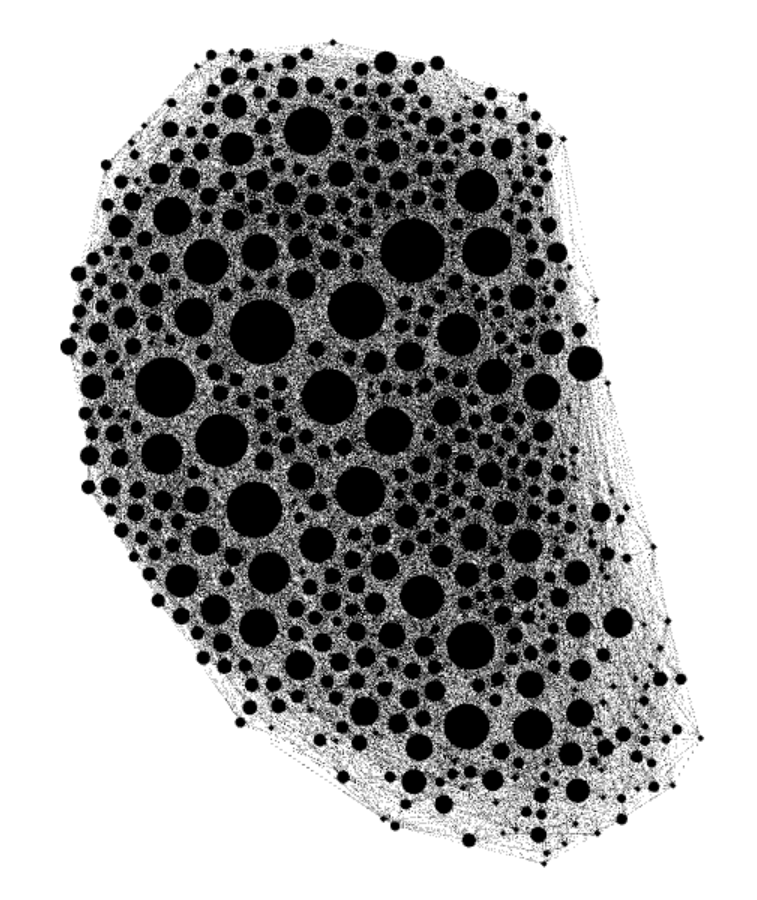
\includegraphics[width=\linewidth]{images/force_atlas.png}
	\end{subfigure}
	\hfill
	\begin{subfigure}{0.48\linewidth}
		\centering
		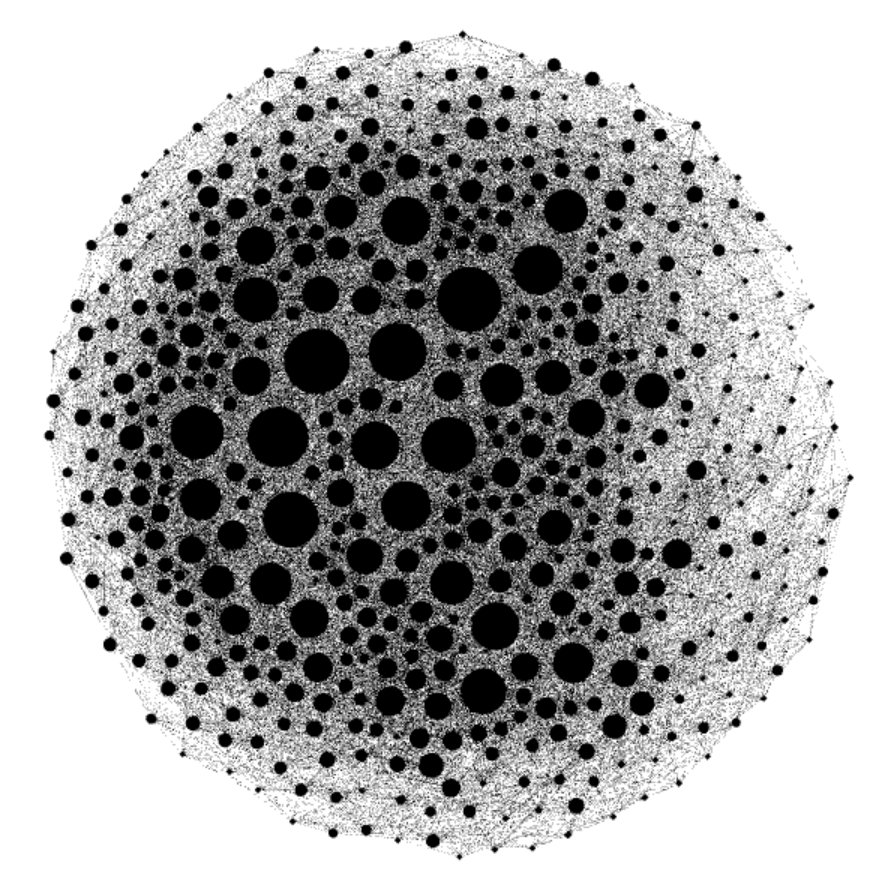
\includegraphics[width=\linewidth]{images/fruchterman.png}
	\end{subfigure}
	\caption{Utilisation des algorithmes Force Atlas (à gauche) et Fruchterman \& Reingold (à droite)}
	\label{fig:algorithmes}
\end{figure}

\subsection{Les outils de réalisation}

Pour réaliser une visualisation en réseaux, il existe plusieurs méthodes. Nous pouvons utiliser des logiciels spécialisés dans la visualisation et l'analyse de réseaux mais il est également possible d'utiliser des bibliothèques JavaScript ou Python. 

\subsubsection{Utilisation d'un logiciel}

Il existe de nombreux logiciels pour visualiser et analyser des réseaux. Certains comme Pajek\footcite{merckleAnalyseReseauxIntroduction2020} ou NodeXL Pro\footcite{NodeXLYourGoto2024} sont propriétaires mais il y en a d'autres qui sont \textit{open-source} tels que Gephi\footcite{GephiOpenGraph} ou Tulip\footcite{tulip-devTulip2025}.

Pour la réalisation de visualisations dans le cadre de l'application AIKON, le logiciel le plus adapté est Gephi en raison de sa simplicité d'utilisation et de son statut \textit{open-source}. Gephi est créé en 2008 par Mathieu Bastian, Sébastien Heymann et Mathieu Jacomy pour donner la possibilité aux chercheurs en sciences humaines de la Fondation de la Maison des Sciences de l'Homme de Paris d'étudier le Web. Aujourd'hui, il existe un consortium Gephi pour collaborer sur le projet avec une communauté internationale\footcite{heymannGephi2014}.

Ce logiciel construit la visualisation à partir de \textit{nodes} et de \textit{edges}. Ces derniers ont des \textit{labels} pour indiquer leur noms ou une autre information pour les identifier. Dans Gephi, il est possible d'importer des fichiers de graphe de type \gls{gexf} et \textit{Gephi project files} ou des fichiers de données tabulaires comme \gls{csv}. Nous pouvons aussi utiliser deux documents \gls{csv}, un pour les \textit{nodes} et un autre pour les \textit{edges}, pour créer une visualisation. 

Une fois le fichier graphe importé, nous pouvons gérer nos données dans le \og Laboratoire de données \fg.

Dans \og Vue d'ensemble \fg, nous pouvons manipuler et analyser notre graphe grâce à différentes fenêtres. La \og Spatialisation \fg permet d'appliquer des algorithmes par modèle de force tels que ceux cités précédemment. Les paramètres de ces derniers comme la gravité ou la force de répulsion sont ajustables. La fenêtre \og Statistiques \fg sert à analyser quantitativement le graphe par exemple en calculant le degré, la modularité ou le coefficient de clustering. La fenêtre \og Aspect \fg permet de modifier l'apparence des \textit{nodes} et des \textit{edges}. Il est possible d'adapter leur taille et leur couleur par rapport à des attributs comme le degré. 

Lorsque nous sommes satisfaits de la disposition de notre graphe, nous pouvons modifier son aspect esthétique dans \og Prévisualisation \fg qui permet de changer la police d'écriture des \textit{labels} ou la forme des \textit{edges} par exemple. 

Ensuite, la visualisation est exportable dans différents formats tels que \gls{gexf} ou \textit{Gephi project files}. Il existe également un module Sigma Exporter qui permet d'exporter le graphe dans un dossier \textit{network} contenant des fichiers \gls{html}, \gls{css} et JavaScript avec la bibliothèque Sigma.js.

\subsubsection{Développement en JavaScript et Python}

Des bibliothèques JavaScript et Python permettent de réaliser, analyser et manipuler des graphes sous la forme de réseaux à partir de fichiers comme \gls{gexf} ou \gls{csv} afin de les intégrer à des pages web. 

En Python, pouvons développer une visualisation en réseaux grâce aux bibliothèques Networkx et Pyvis. En JavaScript, il existe plusieurs bibliothèques pouvant réaliser cette tâche comme amCharts, D3.js et Sigma.js. 

Bien que les visualisations soient particulièrement efficaces pour explorer les relations entre différents éléments d'un corpus, nous pouvons observer parfois une altération ou une perte de données.


